% DRAFT (theory session, 2026-11-05; notes/THEORY_ICML_2026-11.md). Not wired into main.tex.
% Integration needs:
%   \newtheorem{theorem}{Theorem} in main.tex;
%   figs/fig_trap_universality.pdf (figures/theory_icml/fig_trap_universality.py);
%   the appendix paper/sections/appendix_icml.tex (\label{app:trap}).
% Suggested place: a new subsection of Section~\ref{sec:fp} after \S\ref{sec:mechanism}, or a short section after it.
\subsection{The trap obeys a supercritical renewal equation}\label{sec:trap}

Eq.~\eqref{eq:fluid} describes the window, not the trap. In congestion it makes the backlog grow at $\lambda-\lmiss$, but the
registered BURST runs grew at only 18--78\% of that, while still completing 1.13--2.03~$\lref$ (\S\ref{sec:e2},
Appendix~\ref{app:proofs}). The round-robin layer RR of \S\ref{sec:fp-heur} reproduces this numerically, but it is a
heuristic. Here we characterize the trap exactly, within an explicit model of the trapped engine.

In the trap every turn misses, the GPU never idles, and requests are served in the order they join (request-level FCFS;
Proposition~\ref{prop:A}). We therefore model the trapped engine as a fluid FIFO server of unit speed (\emph{model~F}). Turn
$k$ of a session costs $c_k$ all-miss GPU seconds. These costs come from the frozen cost model: the miss prefill of $L_k$
tokens plus the all-miss per-turn decode share, so that $\lmiss=1/\sum_kc_kG_k$ with $G_k=P(T\ge k)$. Sessions arrive at
rate~$\lambda$. A completed turn $k<T$ rejoins the queue at once as turn $k+1$. Tool times of 5\,s against cycles of
minutes are neglected (Appendix~\ref{app:trap}).

A request that joins at $u$ completes at $f(u)=u+V(u)$, where $V$ is the pending work. Call
$u_0, u_1=f(u_0), u_2=f(u_1),\dots$ a \emph{FIFO orbit} and $\Delta_n=u_{n+1}-u_n$ its cycles. Write $\rho=\lambda/\lmiss$.

\begin{theorem}[the trap obeys a renewal equation]\label{thm:trap}
Along every FIFO orbit of model~F the cycles solve the linear renewal recursion
\[
\Delta_n=\sum_{k=1}^{\min(n,K)}\lambda c_kG_k\,\Delta_{n-k}+h_n ,
\]
where $h_n\ge0$, $h_n=0$ for $n\ge K$, and $\sum_nh_n$ is the remaining all-miss work at $u_0$.
\begin{enumerate}[(a),leftmargin=*,nosep]
\item If $\rho<1$, the trap empties after a busy period $V_{\mathrm{tot}}/(1-\rho)$.
\item If $\rho=1$, the backlog stays bounded.
\item If $\rho>1$, let $z>1$ solve $\lambda\sum_kc_kG_kz^{-k}=1$. Then, as $t\to\infty$:
  \begin{itemize}[leftmargin=*,nosep]
  \item the gap between a session's turns grows as $V(t)/t\to z-1$;
  \item the backlog grows as $N(t)/t\to\alpha=\lambda(1-E[z^{-T}])$, and sessions complete at $D=\lambda E[z^{-T}]$;
  \item the sessions present, and the turns served, have the tilted turn mix $G_kz^{-k}/\sum_jG_jz^{-j}$.
  \end{itemize}
\item If $\rho>1$, a session that arrives at time $u$ finishes near $(u+c)z^{T}-c$, where $c=V_{\mathrm{tot}}(0)/(\rho-1)$.
\item As $\rho\downarrow1$, $\alpha/(\lambda-\lmiss)\to E[T]/\bar k_c$, where $\bar k_c=\sum_kkc_kG_k/\sum_kc_kG_k$.
\item If $\rho>1$, the gap becomes proportional to the remaining work, $V=\frac{z-1}{\rho-1}V_{\mathrm{tot}}$ up to a
  geometrically vanishing error. That is, it is proportional to the trap's age counted from its virtual origin
  $-V_{\mathrm{tot}}(0)/(\rho-1)$.
\end{enumerate}
\end{theorem}

\begin{theorem}[youth premium]\label{thm:premium}
In Theorem~\ref{thm:trap}(c), $D/\lmiss=H(z)\,\Gamma(z)$. Here $H(z)=E[T]\,E[z^{-T}]/\sum_kG_kz^{-k}$ depends only on the law of
$T$: it equals 1 for a geometric $T$, and lies in $(1-q^K,1)$ for $T=\min(\mathrm{Geometric}(1-q),K)$. The factor
$\Gamma(z)=E_\nu[c]/E_{\nu^z}[c]$ compares the mean cost of a turn under the stationary mix $\nu_k\propto G_k$ and under the
trapped mix $\nu^z_k\propto G_kz^{-k}$. It is at least 1 and non-decreasing in $z$ whenever costs grow with the turn index.
Near the threshold, $D/\lmiss-1=(\rho-1)(1-E[T]/\bar k_c)+O((\rho-1)^2)$, so the premium is positive close to the threshold
if $\bar k_c>E[T]$ and negative if $\bar k_c<E[T]$.
\end{theorem}

The premium is not automatic, because truncation lowers $H$. With $T=\min(\mathrm{Geometric}(1/15),60)$ and slowly growing
costs, $c_k=1+10^{-3}(k-1)$, it is negative. For our workload, $E[T]/\bar k_c=0.60$--$0.62$ in every cell, so from the
threshold up a trapped engine completes sessions faster than its all-miss capacity. Meanwhile its backlog grows at only about
0.6 of $\lambda-\lmiss$ near the threshold, rising to 0.79 at $\rho\approx6$. In all eight cells the premium is proved positive
for $\rho\ge1.04$. A monotone bracket ($H$ non-increasing, $\Gamma$ non-decreasing, evaluated in floating point) covers
$z\in[1+10^{-12},z_1]$, and the first-order term covers the rest.

\begin{corollary}[what trapped throughput does not tell]\label{cor:trapthr}
In model~F, let the arrival rate change to $\lambda'$ while the trap is busy. The trap then empties if and only if
$\lambda'<\lmiss$, after the busy period $V_{\mathrm{tot}}/(1-\lambda'/\lmiss)$. The threshold is therefore the all-miss
capacity at the \emph{stationary} turn mix, not the throughput $D(\lambda)>\lmiss$ measured in the trap. A cut to any rate in
$(\lmiss, D(\lambda))$ leaves the trap in place: the backlog dips by a few percent and grows again. At exactly $\lmiss$ the
fluid backlog settles at a positive level. A stochastic queue at $\rho'=1$ would eventually empty.
\end{corollary}

\noindent The proofs (Appendix~\ref{app:trap}) are elementary. FIFO and work conservation give
$f(u)=V(0)+W(u)$, with $W$ the work that has joined since time~0. FIFO maps each generation of joins onto the next
generation of completions, which turns the nonlinear fluid into the recursion above, with nonnegative coefficients summing
to~$\rho$. A finite-memory renewal lemma and its Perron root then give the rest. The self-similar regime of
Theorem~\ref{thm:trap}(c)--(d) is not new as a steady solution, with constant flows from the empty state. It is the
single-station case of the steady solutions of fluid FIFO re-entrant lines~\citep{khanin2001steady}. That paper treats
deterministic stages, and its closing remark covers a fixed fraction of the flow leaving at each node. The renewal
recursion adds that every trapped trajectory, from any initial state, converges to this regime, geometrically per
generation and with an explicit virtual origin (part~(f)). Theorem~\ref{thm:premium} and Corollary~\ref{cor:trapthr} are, as far as
we found, new. Model~F is the request-level FCFS analogue of
an overloaded processor-sharing queue, whose branching (Crump--Mode--Jagers) structure is classical
\citep{grishechkin1992processor,jeanmarie1994transient,puha2006overloaded}. The paper's layer RR is the processor-sharing
version; its growth differs from model~F's by about 2\%. Lu et al.\ state that arrivals below their low-reuse departure
rate drain the population, and that the throughput measured in a trap sets the scale of the cut
needed~\citep{lu2026cachetrap}. Corollary~\ref{cor:trapthr} sharpens this for FIFO traps: the measured throughput exceeds
the drain threshold, consistent with their simulations, which recovered only below the trapped departure rate. We do not
prove that the engine converges to model~F.

\begin{figure*}[t]\centering
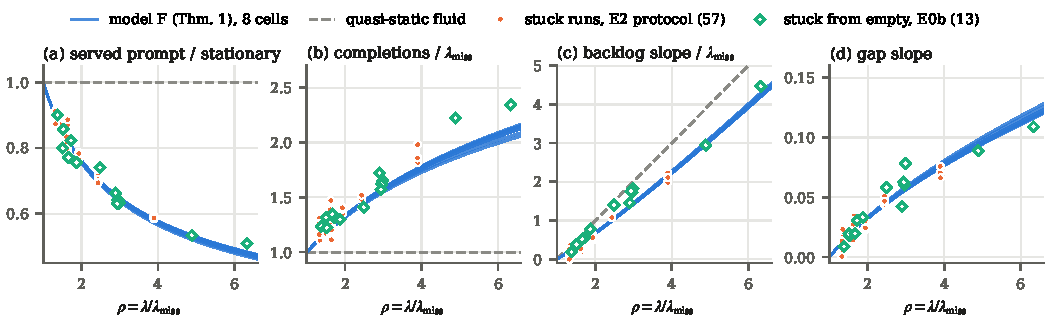
\includegraphics[width=\textwidth]{figs/fig_trap_universality.pdf}
\caption{Theorem~\ref{thm:trap} against every stuck run, as a function of the load $\rho=\lambda/\lmiss$. Points are
measured in the 57 stuck runs of the E2 protocol (orange) and the 13 runs that lost the good state from empty (E0b,
hollow). Lines are model~F for each of the eight cells; they nearly coincide, as Corollary~\ref{cor:trapinv}
(Appendix~\ref{app:trap}) predicts. No parameter is fitted to any trap measurement. (a)~Mean prompt of the turns served, over the stationary mean:
the tilted turn mix. (b)~Session completion rate over $\lmiss$: the youth premium, above 1. (c)~Backlog growth over
$\lmiss$. (d)~Growth rate of the gap between a session's turns, $\gamma=z-1$. The dashed lines show the quasi-static
fluid read literally in congestion: stationary composition, completion at $\lmiss$, growth at $\rho-1$. The paper's layer RR
already corrects (c) numerically.}\label{fig:trapuniv}
\end{figure*}

\begin{table}[t]
\centering\footnotesize
\caption{Theorem~\ref{thm:trap} against every stuck run of the E2 protocol (follow-up hit fraction below 0.2 over the
window $[5700,8700)$\,s), per seed (vLLM: the registered and exploratory runs, which share plans). No parameter is fitted to
any trap measurement; vLLM, the H200 and Llama take one speed factor fitted to their E0a token rate. $\rho=\lambda/\lmiss$ uses
the model's $\lmiss$. $\bar L$: mean prompt of the turns served, measured, against the tilted-mix prediction (the stationary
mean is about 10{,}500). Gap slope: the trend of the median gap between a session's turns, against $\gamma=z-1$. $D$: the
session completion rate, as a multiple of $\lref$. Backlog: the slope as a fraction of $\lambda-\lref$, against
$\alpha/(\lambda-\lmiss)$. The heuristic layer RR gave 0.64 and 0.63 at 300k. Full table, E0b runs and pool sweep:
Appendix~\ref{app:trap}, \fpath{results/theory/icml/trap_check.md}.}\label{tab:trap}
\setlength{\tabcolsep}{1.6pt}
\resizebox{\columnwidth}{!}{%
\begin{tabular}{@{}l c c c c c@{}}
\toprule
cell, rate & $\rho$ & $\bar L$ meas.\ / pred. & gap slope / $\gamma$ & $D/\lref$ / pred. & backlog / pred.\\
\midrule
300k 1.35 & 1.34 & 9125--9556 / 9324 & .004--.020 / .013 & 1.13--1.28 / 1.13 & .14--.89 / .63\\
300k 1.65 & 1.64 & 8417--8830 / 8606 & .015--.027 / .023 & 1.25--1.35 / 1.23 & .59--.78 / .65\\
native 2.5 & 2.44 & 7264--7484 / 7374 & .044--.051 / .045 & 1.44--1.56 / 1.49 & .74--.79 / .69\\
native 4.0 & 3.90 & 6127--6213 / 6115 & .066--.076 / .081 & 1.87--2.03 / 1.81 & .68--.76 / .74\\
vLLM 1.35 & 1.32 & 9097--9547 / 9393 & .000--.016 / .012 & 1.18--1.28 / 1.14 & .00--.74 / .63\\
vLLM 1.65 & 1.62 & 8104--8778 / 8676 & .013--.028 / .022 & 1.30--1.42 / 1.24 & .41--.80 / .65\\
H200 1.5 & 1.45 & 9015--9177 / 9062 & .015--.022 / .017 & 1.20--1.27 / 1.20 & .49--.78 / .64\\
H200 2.0 & 1.93 & 8058--8230 / 8082 & .023--.031 / .032 & 1.40--1.45 / 1.36 & .51--.66 / .66\\
Llama 1.35 & 1.33 & 9075--9512 / 9356 & .003--.016 / .013 & 1.22--1.33 / 1.14 & .00--.75 / .64\\
Llama 1.65 & 1.63 & 8459--8757 / 8631 & .013--.021 / .023 & 1.34--1.49 / 1.23 & .29--.63 / .66\\
\bottomrule
\end{tabular}}
\end{table}

\paragraph{Against the engine (retrospective).} Table~\ref{tab:trap} tests Theorem~\ref{thm:trap} on every stuck run of the
registered protocol, with no parameter fitted to any trap measurement:
\begin{itemize}[leftmargin=*,nosep]
\item \emph{Composition.} The mean prompt of the turns served matches the tilted mix to within $-6.6$\% and $+7.7$\% in all
57 stuck runs of the E2 protocol, and to within 3\% in 50 of them. In these runs the prediction ranges from 6{,}115 to
9{,}393 tokens. The trapped engine serves a young backlog of short turns, which the paper noted; the theorem says how young.
\item \emph{Cycle growth.} The gap between a session's turns, the quantity whose median Table~\ref{tab:gapR} reports,
grows in time at slope $\gamma$. Measured over predicted, the ratio has median 0.98.
\item \emph{Youth premium.} Every stuck run completes sessions above $\lref$, at 1.10--2.40~$\lref$, and on average 5\%
above~$D$; the congested engines run a few percent above E0a's reference rate (Appendix~\ref{app:proofs}).
\item \emph{Backlog.} The backlog grows at 0.63 of $\lambda-\lref$ on average, the value the heuristic layer RR gave
numerically at 300k.
\end{itemize}
The same law holds for the 13 runs that lost the good state from empty (E0b), from $\rho=1.4$ to~6.3, on the pool sweep
and on the H200 (Appendix~\ref{app:trap}).

The theorem also explains the registered slope rule's fragility at the lower rate. That rule calls a run trapped if its
backlog slope exceeds $0.5(\lambda-\lref)$, while the true slope is only about $0.63(\lambda-\lmiss)$. A seed whose arrival
plan dips by a few percent over the evaluation window can therefore fall below the line. Because the plans are common random
numbers, seed~1's plan dips below nominal in every cell and rate, by 5.8--8.9\% at 1.35~$\lref$. Eight of the nine runs whose
slope fell below the threshold are seed~1. A plug-in prediction computable from the plan before any run,
$\lambda_{\mathrm{window}}(\text{plan})-D$, falls on the measured side of the threshold for 27 of the 30 independent plans
of the registered protocols. Always predicting ``trapped'' scores 23. Two of the three misses lie within $10^{-4}$\,/s of
the threshold; the third is Llama at 1.35~$\lref$, the registered failure. The account is post hoc and changes no verdict.

Predictions for runs that did not yet exist (trapped composition, cycle slope, completion rate, backlog slope, and per-seed
slope-test outcomes) were frozen under tag \texttt{icml-trap-pred} (Appendix~\ref{app:trap}).
